\subsection{Experiment 7B: family-informed personalization}
\label{sec:experiment7b}

\paragraph{Reason for the revised sequence.}
Experiment 7A fails the collaboration gate because accurate local fits
outperform fixed family pooling. Consequently, the originally envisaged next
step of federated estimation is deferred. Experiment 7B instead tests the
personalization diagnostic proposed in \cref{sec:experiment7a}: can a family
prior help local estimation without forcing different clients to share the
same parameters? The failed 7A result is retained. This experiment remains
centralized and uses oracle family labels.

\paragraph{Unchanged data regime and new fleets.}
The protocol uses ten new realizations, seeds 41--50, with 30 clients each.
It retains the primary 7A regime: three two-second constant-speed episodes,
restricted speed anchors, sideslip-proxy noise of 0.05 degrees, and yaw-rate
noise of 0.1 degrees/s. Family separation, client scatter, nominal collection
controller, references, known initial state, and exact speed and steering are
unchanged. Neither noise nor scarcity is increased after observing 7A.
The same three held-out 24-second scenarios and corrected tanh-tire plant are
used for evaluation. These fleets are independent of 7A; within each fleet,
test trajectories belong to the same physical clients as identification.

\paragraph{Family prior without validation leakage.}
For client $i$, first fit $\bar p_{c,-i}$ using only the other nine members
of its true family. No record from client $i$ contributes to this prior.
This gives a fixed donor prior for all of the client's validation folds.
Using the 7A output predictor and scales, the personalized estimate is
\begin{equation}
 \hat p_i(\lambda;\mathcal D)=\arg\min_{p\in\mathcal P}
 \frac{1}{2N_{\mathcal D}}\sum_{d,k}
 \left\|W\big(\hat y_{d,k}(p)-y_{d,k}\big)\right\|_2^2
 +\lambda\left\|\frac{\log p-\log\bar p_{c,-i}}{0.05}\right\|_2^2,
 \label{eq:7bobjective}
\end{equation}
where $N_{\mathcal D}$ counts transitions, so $2N_{\mathcal D}$ counts scalar
output residuals. The logarithm acts componentwise and $\mathcal P$ is the
same positive bounded parameter domain as in 7A. The fixed 0.05 log scale
sets the penalty units; it is not an estimated prior standard deviation.
Normalizing the data term makes the meaning of $\lambda$ consistent between
four-second fold fits and the six-second final fit. The implementation
multiplies the whole objective by the number of scalar residuals and appends
the resulting prior residuals to the least-squares problem. At $\lambda=0$,
it exactly preserves the unregularized fitting objective and implementation.
Both solver starts and tolerances are unchanged.

\paragraph{Selection using identification records only.}
The candidate strengths are fixed before execution:
\begin{equation}
 \Lambda=\{0,10^{-3},10^{-2},10^{-1},1,10\}.
\end{equation}
For each candidate, fit on two complete episodes and predict the third from
its known zero initial state. Repeat for all three held-out episodes and
select the smallest average standardized output error. Ties select the lower
strength. This validates free-run prediction, not closed-loop tracking.
The selected strength is then used to refit on all three local episodes.
If zero is selected, the final Local fit is reused exactly. No additional
validation recordings are supplied and no test trajectory, true parameter,
or test tracking metric enters selection. Since validation episodes contain
different speed anchors, the selection also probes prediction beyond the
two fitting anchors within the client's assigned interval.

\paragraph{Comparisons and resource accounting.}
\textbf{Local} fits all six seconds from each client independently.
\textbf{Family} fits one shared model to all ten clients' six-second records
in each true family. \textbf{Personalized} uses the donor prior and selected
local estimate in \cref{eq:7bobjective}. Family pooling remains an exact
comparison to the deployed family architecture in 7A, whereas the prior
excludes the recipient specifically to protect validation integrity.
All methods access the same recorded fleet dataset. Each donor prior uses
54 seconds, each Family fit 60 seconds, and each Local final fit six seconds.
Each validation candidate uses four local seconds for fitting and two for
scoring. Personalization increases fitting effort and deploys 30 model and
controller families, just as Local does; it does not inherit Family's
three-family deployment advantage. The leave-one-client-out priors are a
diagnostic construction, not an efficient federated implementation.

\paragraph{Evaluation and decision rule.}
The common LQI weights, gain grid, held-out prediction inputs, amplitude
checks, and 161-speed frozen audit are retained. The primary gate requires
Personalized to improve fleet-average tracking relative to Local by at least
5\%, with a positive lower 95\% paired bootstrap bound, amplitude feasibility,
and frozen spectral radius below one. The ten fleet seeds are the independent
units; bootstrap uses 10,000 draws and seed 7201. Comparisons against Family,
worst-family tracking, parameter error, common-input prediction, and selected
strength counts are secondary diagnostics. Lower cross-validation error alone
does not constitute held-out improvement, since it is the selection objective.

\paragraph{Results and interpretation.}
All 6,284 fits, including the 5,400 validation fits, converge from both starts
without bound hits. Final fits are reused for the 46 clients selecting zero
regularization. The maximum multistart relative parameter difference is
$4.44\times10^{-7}$. All 2,700 closed-loop evaluations satisfy amplitude
limits and the largest frozen spectral radius is 0.96933. These checks do not
constitute a formal varying-speed stability guarantee.

\begin{table}[htbp]
\centering
\caption{Experiment 7B on ten new fleets: six seconds of noisy restricted
local data. Tracking reports mean $\pm$ standard deviation across fleet seeds.
Parameter error uses the same componentwise relative-error convention as 7A.}
\label{tab:experiment7b}
\begin{tabular}{lrrr}
\toprule
Method & Tracking [deg/s] & Yaw prediction [deg/s] & Parameter error\\
\midrule
Local & $0.006669\pm0.000016$ & 0.04667 & 0.787\%\\
Family & $0.007651\pm0.000368$ & 0.15837 & 2.627\%\\
Personalized & $0.006672\pm0.000017$ & 0.04637 & 0.842\%\\
\bottomrule
\end{tabular}
\end{table}

\begin{figure}[htbp]
\centering
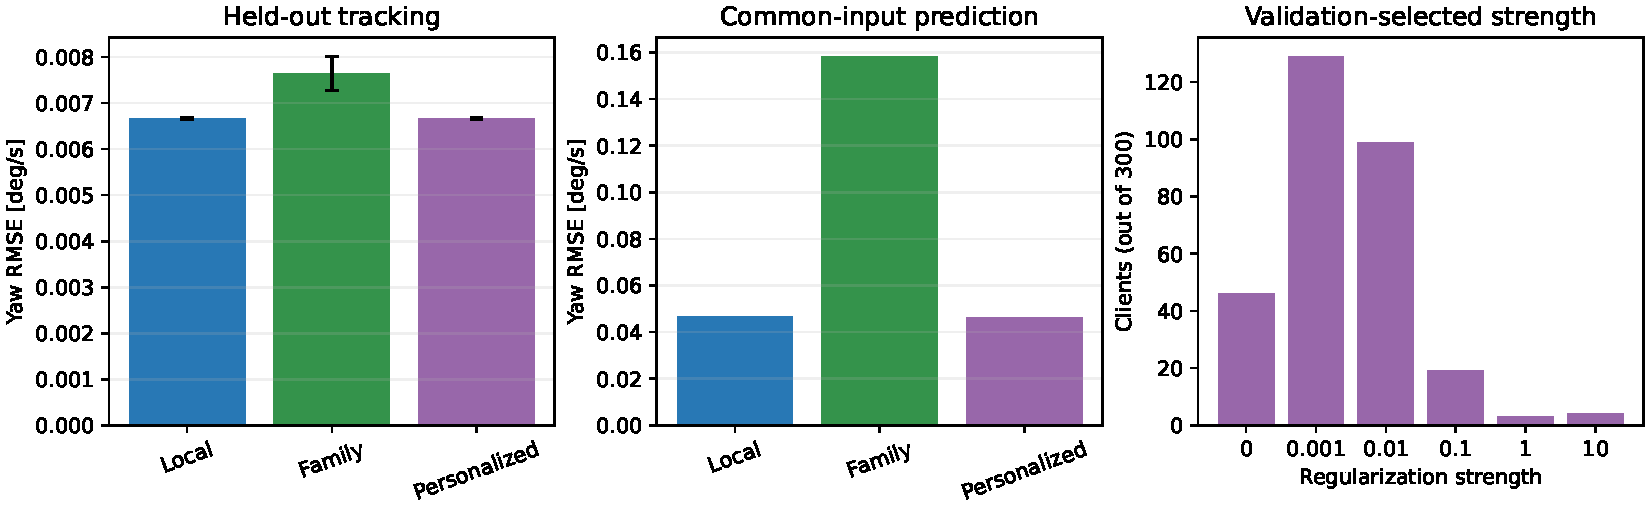
\includegraphics[width=\linewidth]{../results/figures/experiment_7b_personalization.pdf}
\caption{Experiment 7B: held-out tracking, common-input yaw prediction, and
the distribution of validation-selected regularization strengths. Tracking
error bars show standard deviation across ten fleets. Prediction and tracking
use different inputs and should not be compared in absolute magnitude.}
\label{fig:experiment7b}
\end{figure}

\Cref{tab:experiment7b,fig:experiment7b} shows that personalization nearly
recovers Local performance while improving tracking over Family by 12.79\%.
Against Local, however, tracking error increases by 0.0573\%. The paired
difference $J_{\rm Local}-J_{\rm Personalized}$ is
$-3.82\times10^{-6}$ deg/s, with 95\% bootstrap interval
$[-7.37\times10^{-6},-1.65\times10^{-7}]$ deg/s. Three of ten fleet pairs
favor Personalized. The primary 5\% improvement gate therefore fails.
The absolute penalty is tiny, so the practical conclusion is near-parity,
with no demonstrated tracking improvement, rather than a substantial
personalization failure.

The selected-strength counts for $\lambda=0,0.001,0.01,0.1,1,10$ are
46, 129, 99, 19, 3, and 4, respectively. Thus 274 of 300 clients select at
most 0.01. This supports weak shrinkage in this setting; it does not show
that those strengths are optimal outside the tested grid or data regime.
The four upper-end selections are retained without expanding the grid after
seeing test outcomes. Common-input yaw prediction improves by only 0.64\%
relative to Local, with paired difference interval
$[-0.000187,0.000808]$ deg/s spanning zero. Relative parameter error increases
from 0.787\% to 0.842\%. Neither secondary result establishes a reliable
estimation advantage. Worst-family tracking is likewise nearly unchanged,
0.006805 versus 0.006808 deg/s. Steering RMS is approximately 0.80852 degrees
for both, with peak rates about 1.1693 degrees/s.

\paragraph{What this establishes and what remains open.}
Forcing all family members to use one estimate causes a measurable penalty,
and allowing local parameters largely removes it. Nevertheless, the strong
three-ratio structure and available state observations already allow accurate
local identification. A donor prior has little estimation uncertainty to
remove here, while it can still introduce client mismatch. This interpretation
is consistent with 7A's clean-data and data-length contrasts, although 7B does
not provide a formal bias--variance decomposition. Prediction-based validation
also need not minimize downstream tracking error.

Experiments 7A and 7B therefore do not yet justify a claim of federated accuracy
improvement. Fixed family sharing has a deployment-complexity trade-off;
personalization retains 30 controllers and recovers local accuracy. Those are
distinct findings. The next decision should be whether the intended application
actually has a local information limitation absent here, such as unavailable
sideslip measurements or insufficient excitation. Such an assumption must be
motivated and specified before a new experiment. Further tuning of this
regularization grid or increasing noise solely to obtain a positive result
is not the default next step. Federated optimization and learned clustering
remain deferred.

\paragraph{Reproducibility.}
The protocol is \path{code/config/experiment_7b.json}. The runner is:
\begin{quote}\small
\path{code/experiments/experiment_7b_personalization.py}
\end{quote}
Set \texttt{PYTHONPATH=code/src}. The \texttt{--summarize-only} option rebuilds
the aggregates and figure. Compressed per-seed outputs retain every fold's
candidate parameters, validation loss and solver diagnostics, selected strengths,
final fits, donor identities, identification-data hashes, and held-out metrics.
The conclusions file records protocol and implementation hashes.
The 38-test suite includes exact preservation at zero regularization, approach
to the prior under a dominant penalty, explicit episode exclusion in validation,
and rejection of an incorrect prior on clean identifiable data.
